% fig_regime_map.tex
% Current multiple M vs fault resistance Rf with three operating regimes
% Curves: 3PH (solid blue), SLG (dashed red)
% Regime bands: instantaneous (green), inverse-time HIF (orange), no-trip (red)
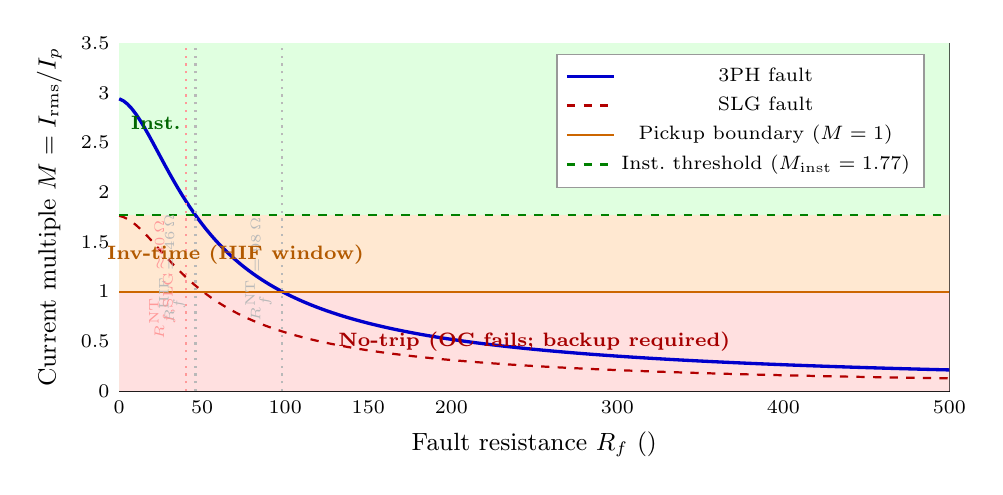
\begin{tikzpicture}
\begin{axis}[
  width=\columnwidth, height=6.0cm,
  xlabel={Fault resistance $R_f$ (\si{\ohm})},
  ylabel={Current multiple $M = I_{\mathrm{rms}}/I_p$},
  xmin=0, xmax=500,
  ymin=0, ymax=3.5,
  xtick={0,50,100,150,200,300,400,500},
  ytick={0,0.5,1.0,1.5,2.0,2.5,3.0,3.5},
  minor tick num=1,
  grid=both,
  grid style={gray!25,line width=0.3pt},
  minor grid style={gray!12,line width=0.2pt},
  tick label style={font=\scriptsize},
  label style={font=\small},
  legend style={at={(0.97,0.97)},anchor=north east,
                font=\scriptsize,fill=white,draw=black!40,
                inner sep=3pt},
  clip=false]

  % ---- Shaded regime bands ----
  % No-trip (M < 1)
  \addplot[fill=red!12,draw=none,forget plot]
    coordinates {(0,0)(500,0)(500,1.0)(0,1.0)} \closedcycle;
  % Inverse-time HIF window (1 < M < 1.77)
  \addplot[fill=orange!18,draw=none,forget plot]
    coordinates {(0,1.0)(500,1.0)(500,1.77)(0,1.77)} \closedcycle;
  % Instantaneous (M > 1.77)
  \addplot[fill=green!12,draw=none,forget plot]
    coordinates {(0,1.77)(500,1.77)(500,3.5)(0,3.5)} \closedcycle;

  % ---- M(Rf) for 3PH ----
  % M_3ph = (V0/sqrt(2)/Ip) * 1/sqrt((Ra+Rth+Rf_pu)^2 + (Xd''+Xth)^2)
  % Base: 121 Ohm.  Ip=0.8, V0=1.0
  % M = 0.8839 / sqrt((0.02+Rf/121)^2 + 0.09)
  \addplot[blue!80!black,very thick,samples=200,domain=0:500]
    { 0.8839 / sqrt( (0.02 + x/121)^2 + 0.09 ) };
  \addlegendentry{3PH fault}

  % ---- M(Rf) for SLG ----
  % SLG: positive-sequence component approx 0.60 of 3PH for this system
  \addplot[red!70!black,thick,dashed,samples=200,domain=0:500]
    { 0.530 / sqrt( (0.02 + x/121)^2 + 0.09 ) };
  \addlegendentry{SLG fault}

  % ---- Regime boundary lines ----
  \addplot[orange!80!black,thick,domain=0:500]
    coordinates {(0,1.0)(500,1.0)};
  \addlegendentry{Pickup boundary ($M=1$)}

  \addplot[green!50!black,thick,dashed,domain=0:500]
    coordinates {(0,1.77)(500,1.77)};
  \addlegendentry{Inst.\ threshold ($M_{\mathrm{inst}}=1.77$)}

  % ---- Vertical regime markers ----
  \draw[gray!55,thick,dotted]
    (axis cs:46,0) -- (axis cs:46,3.5)
    node[above,font=\tiny,gray!55,rotate=90,pos=0.35]
    {$R_f^{\mathrm{HIF}}=46\,\Omega$};
  \draw[gray!55,thick,dotted]
    (axis cs:98,0) -- (axis cs:98,3.5)
    node[above,font=\tiny,gray!55,rotate=90,pos=0.35]
    {$R_f^{\mathrm{NT}}=98\,\Omega$};

  % SLG no-trip boundary
  \draw[red!40,thick,dotted]
    (axis cs:40,0) -- (axis cs:40,3.5)
    node[above,font=\tiny,red!40,rotate=90,pos=0.32]
    {$R_{f,\mathrm{SLG}}^{\mathrm{NT}}{\approx}40\,\Omega$};

  % ---- Region text labels ----
  \node[font=\scriptsize\bfseries,green!40!black,align=center]
    at (axis cs:22,2.7) {Inst.};
  \node[font=\scriptsize\bfseries,orange!70!black]
    at (axis cs:70,1.37) {Inv-time (HIF window)};
  \node[font=\scriptsize\bfseries,red!65!black]
    at (axis cs:250,0.5) {No-trip (OC fails; backup required)};

\end{axis}
\end{tikzpicture}
